\documentclass{article}
\usepackage{enumitem}
\usepackage{graphicx}
\usepackage{subcaption}
\usepackage{tikz}
\usepackage{adjustbox}
\usetikzlibrary{tikzmark}

\begin{document}

\section{Autonomous Landing System}
\textbf{Draven} software enables it to land to specsifiied spot autonomously through the utilization of advanced image processing techniques and ROV control. 
Using the \textbf{Motion Decision Block} processes input frames from the camera to identify the designated landing spot. The resulting processed frame is then forwarded to the Decision Making Algorithm, which estimates the relative distance from the camera's position to the identified spot. 
Subsequently,the Decision Making Algorithm generates $(X,Y,Z)$ coordinates, indicating the direction of movement based on the estimated distance. These coordinates serve as input for a closed-loop control system.The Control Block, equipped with a PID Controller, computes and guides the ROV's movements, stabilizing and smoothing its motion to navigate effectively within the surrounding environment as it overcome the effect of it on the motion.
%==============================================
%                  BEGIN FIGURE
%==============================================

\begin{figure}[h]
    \begin{adjustbox}{width=1.3\textwidth,center}
    \begin{tikzpicture}
        % First figure
        \node[draw, rectangle, blue, fill= blue!10, text width=50pt,align=center] (parent_figure1) at (0,0) {Reading Camera Frame};

        % Second figure
        \node[draw, rectangle, blue, fill= blue!20] (parent_figure2) at (5,0) {
        
        \begin{tikzpicture}
        %  figure
        \node[draw, rectangle, blue, fill= blue!10, text width=50pt,align=center] (child_figure1) at (4,0) {Detection and Preprocessing};

        %  figure
        \node[draw, rectangle, blue,fill= blue!10, text width=50pt,align=center] (child_figure2) at (7,0) {Decision Making Algorithm};

        \draw[->, line width=1.3pt, blue] (child_figure1) -- (child_figure2);
        
        \end{tikzpicture}
        };
        \node[above=25pt, text width=100pt,align=center, blue!70] at (parent_figure2) {Motion Decision Block};

        % Second figure
        \node[draw, rectangle, blue, fill= blue!20] (parent_figure3) at (11,0) {
        
        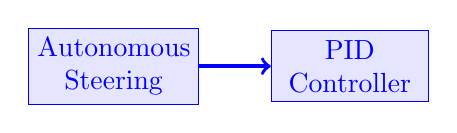
\begin{tikzpicture}
        % figure

        \node[draw, rectangle, blue,fill= blue!10,text width=55pt,align=center] (child_figure3) at (11,0) {Autonomous Steering};

        \node[draw, rectangle, blue,fill= blue!10, text width=50pt,align=center] (child_figure4) at (14,0) {PID Controller};

        % Third figure
        \draw[->, line width=1.3pt, blue] (child_figure3) -- (child_figure4);
        \end{tikzpicture}
        };
        \node[above=25pt, text width=100pt,align=center, blue!70] at (parent_figure3) {Control Block};


        % Arrow between figures
        \draw[->, line width=1.3pt, blue] (parent_figure1) -- (parent_figure2);
        \draw[->, line width=1.3pt, blue] (parent_figure2) -- (parent_figure3);

        \draw[->, line width=1.3pt, blue] (parent_figure3) to[bend right] (parent_figure1);

    \end{tikzpicture}
    \end{adjustbox}
    \caption{Autonomous system flow chart}
    \label{fig:Autonomous_system}
    \end{figure}

%==============================================
%                  END FIGURE
%==============================================
  
%==============================================
%                  BEGIN FIGURE
%==============================================
\subsection{Motion Decision Block}
The Motion Decision Block software consists of multiple sequential stages. The first stage involves processing the input frame through a Color Detection and Noise Reduction Algorithm, which serves to isolate the Region Of Interest (in this case, the landing spot) from the surrounding environment. 
Following this, the ROI is thresholded to be further processed by the Bounding Box Coordinates node, which allocates the ROI in the frame using the $(X1,Y1,X2,Y2)$ coordinates. 
These coordinates are then fed to the Decision Making Algorithm, which estimates the relative distance from the ROV to the Landing Spot and further produces the ROV motion presented in $(X,Y,Z)$ coordinates, as shown in Figure \ref{fig:decision}
\begin{figure}[htbp]
    \centering
    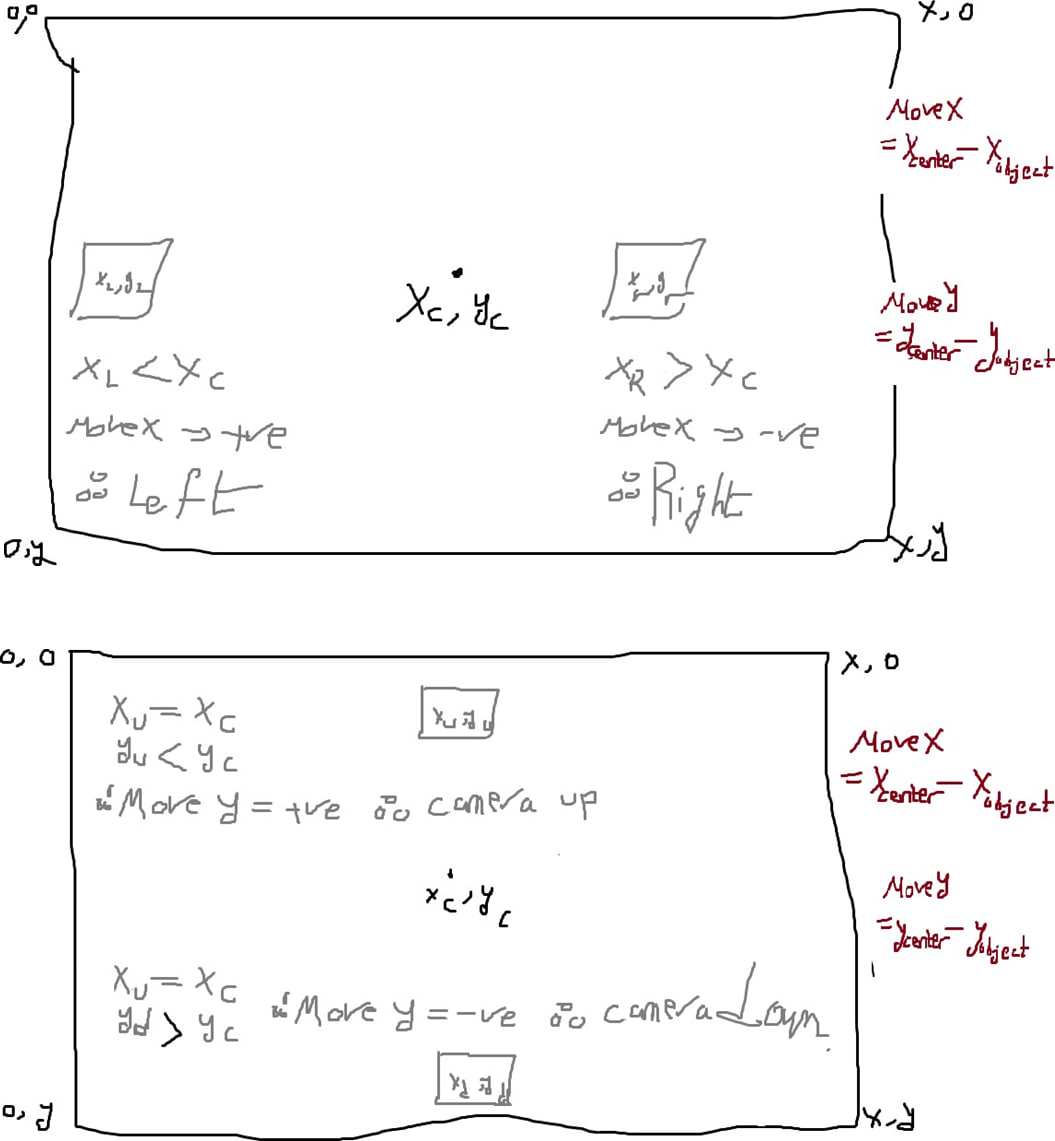
\includegraphics[width=0.7\textwidth]{images/motion.jpg}
    \caption{Figure illustrates how the Decision Making Algorithm works with respect to the presence of the ROI in the frame.}
    \label{fig:decision}
\end{figure}

\begin{figure}[h]
\begin{adjustbox}{width=1.3\textwidth,center}
    \begin{tikzpicture}

    \node[draw, rectangle, blue, fill= blue!10] (first) at (0,0) {
    \begin{tikzpicture}
        % First figure
        \node[draw, rectangle, blue, fill= blue!20] (figure1) at (0,0) {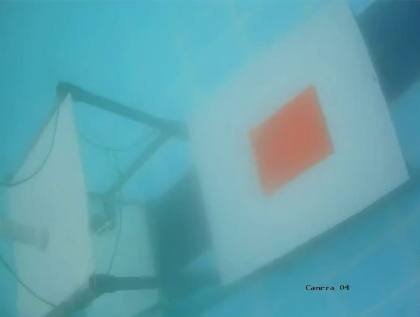
\includegraphics[width=0.2\textwidth]{images/inputjpg.jpg}};
        \node[above=50pt, text width=100pt,align=center] at (figure1) {Input Frame};

        % Second figure
        \node[draw, rectangle, blue, fill= blue!20] (figure2) at (3,0) {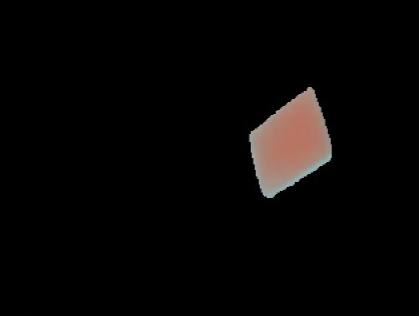
\includegraphics[width=0.2\textwidth]{images/color_thre.jpg}};
        \node[above=50pt, text width=100pt,align=center] at (figure2) {ROI detection and noise reduction};

        % Second figure
        \node[draw, rectangle, blue, fill= blue!20] (figure3) at (6,0) {
\includegraphics[width=0.2\textwidth]{images/thre.jpg}};
        \node[above=50pt, text width=100pt,align=center] at (figure3) {ROI thresholding};

        % Third figure
        \node[draw, rectangle, blue, fill= blue!20] (figure4) at (9,0) {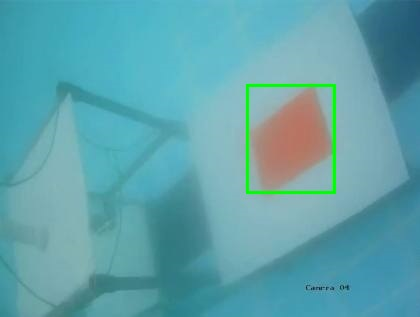
\includegraphics[width=0.2\textwidth]{images/bbox.jpg}};
        \node[above=50pt,text width=100pt,align=center] at (figure4) {ROI Bounding Box Coordinates};

        % Arrow between figures
        \draw[->, line width=1.3pt, blue] (figure1) -- (figure2);
        \draw[->, line width=1.3pt, blue] (figure2) -- (figure3);
        \draw[->, line width=1.3pt, blue] (figure3) -- (figure4);
    
    \end{tikzpicture}
    };
    \node[above=70pt, text width=140pt,align=center, blue!70] at (first) {Detection and Preprocessing};
    
    % figure
    \node[draw, rectangle, blue, fill= blue!20] (second) at (9,0) {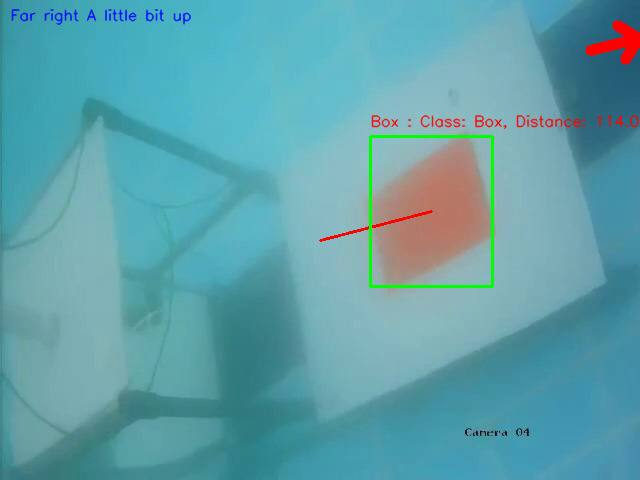
\includegraphics[width=0.25\textwidth]{images/decision.jpg}};
    \node[above=70pt, text width=140pt,align=center, blue!70] at (second) {Decision Making Algorithm};

    % Arrow between figures
    \draw[->, line width=1.3pt, blue] (first) -- (second);

  \end{tikzpicture}
  \end{adjustbox}
  \caption{Motion Decision Block}
  \label{fig:Motion Decision}
  \end{figure}

%==============================================
%                  END FIGURE
%==============================================

\end{document}
